% 设定文章类型,正文字号为五号,若需小四将5改为-4即可
\documentclass[zihao=5,UTF8]{report}		


% 文章宏定义
\def\N{\mathbb{N}}
\def\F{\mathbb{F}}
\def\Z{\mathbb{Z}}
\def\Q{\mathbb{Q}}
\def\R{\mathbb{R}}
\def\C{\mathbb{C}}
\def\T{\mathbb{T}}
\def\S{\mathbb{S}}


\def\A{\mathbb{A}}
\def\I{\mathscr{I}}
\def\d{\mathrm{d}}
\def\p{\partial}


% 导入基本宏包
\usepackage[UTF8]{ctex}     % 设置文档为中文语言
\usepackage[colorlinks,linkcolor=blue,anchorcolor=blue,citecolor=blue,urlcolor=blue]{hyperref}   %(此宏包与标题中的数学环境冲突)  % 宏包:自动生成超链接
% \usepackage{docmute}    % 宏包:子文件导入时自动去除导言区,用于主/子文件的写作方式,\include{./51单片机笔记}即可。注:启用此宏包会导致.tex文件capacity受限。
\usepackage{amsmath}    % 宏包:数学公式
\usepackage{mathrsfs}   % 宏包:提供更多数学符号
\usepackage{amssymb}    % 宏包:提供更多数学符号
\usepackage{pifont}     % 宏包:提供了特殊符号和字体
\usepackage{extarrows}  % 宏包:更多箭头符号
\usepackage{tabularray} % 宏包:更多表格设置
\usepackage{booktabs}   % 宏包:更多表格设置
\usepackage{longtable}  % 宏包:更多表格设置
% 文章页面margin设置
\usepackage[a4paper]{geometry}
\geometry{top=1in}
\geometry{bottom=1in}
\geometry{left=0.75in}
\geometry{right=0.75in}   % 设置上下左右页边距
\geometry{marginparwidth=1.75cm}    % 设置边注距离(注释、标记等)

% theorem环境自定义
\usepackage{amsthm}
\newtheoremstyle{MyTheoremStyle}% <name>
    {11pt}% <space above>
    {11pt}% <space below>
    {}% <body font> 使用默认正文字体
    {}% <indent amount>
    {\bfseries}% <theorem head font> 设置标题项为加粗
    {:\\ }% <punctuation after theorem head>
    {.5em}% <space after theorem head>
    {\textbf{#1}\thmnumber{#2}\ \ (\,\textbf{#3}\,)}% 设置标题内容顺序
\theoremstyle{MyTheoremStyle} % 应用自定义的定理样式
\newtheorem{theorem}{Theorem.\,}

% definition 环境自定义
\newtheoremstyle{MySubsubsectionStyle}% <name>
    {11pt}% <space above>
    {11pt}% <space below>
    {}% <body font> 使用默认正文字体
    {}% <indent amount>
    {\bfseries}% <theorem head font> 设置标题项为加粗
    {:\\ \indent}% <punctuation after theorem head>
    {0pt}% <space after theorem head>
    {\textbf{#3}}% 设置标题内容顺序
\theoremstyle{MySubsubsectionStyle} % 应用自定义的定理样式
\newtheorem{definition}{}

%宏包:有色文本框及其设置
\usepackage[dvipsnames,svgnames]{xcolor}    %设置插入的文本框颜色
\usepackage[strict]{changepage}     % 提供一个 adjustwidth 环境
\usepackage{framed}     % 实现方框效果
\definecolor{graybox_color}{rgb}{0.95,0.95,0.96} % 文本框颜色。修改此行中的 rgb 数值即可改变方框纹颜色,具体颜色的rgb数值可以在网站https://colordrop.io/ 中获得。(截止目前的尝试还没有成功过,感觉单位不一样)(找到喜欢的颜色,点击下方的小眼睛,找到rgb值,复制修改即可)
\newenvironment{graybox}{%
\def\FrameCommand{%
\hspace{1pt}%
{\color{gray}\small \vrule width 2pt}%
{\color{graybox_color}\vrule width 4pt}%
\colorbox{graybox_color}%
}%
\MakeFramed{\advance\hsize-\width\FrameRestore}%
\noindent\hspace{-4.55pt}% disable indenting first paragraph
\begin{adjustwidth}{}{7pt}%
\vspace{2pt}\vspace{2pt}%
}
{%
\vspace{2pt}\end{adjustwidth}\endMakeFramed%
}

% chapter标题自定义设置
\usepackage{titlesec}   
\titleformat{\chapter}[hang]{\normalfont\huge\bfseries\centering}{第\,\thechapter\,章}{20pt}{}
\titlespacing*{\chapter}{0pt}{-20pt}{20pt} % 控制上方空白的大小
% section标题自定义设置 
\titleformat{\section}[hang]{\normalfont\Large\bfseries}{§\,\thesection\,}{8pt}{}
% subsubsection标题自定义设置
%\titleformat{\subsubsection}[hang]{\normalfont\bfseries}{}{8pt}{}


% table设置
\usepackage{float}
\usepackage{booktabs}
\usepackage{caption}

%宏包:图片插入设置
\usepackage{graphicx}   
\usepackage{float}      
\usepackage{amssymb}    
\usepackage{caption}
\captionsetup[figure]{name=图}  
\captionsetup[table]{name=表}
\captionsetup{
            labelfont=bf, % 设置标签为粗体
            textfont=bf,  % 设置文本为粗体
            font=small  
        }

% 文章默认字体设置
\usepackage{fontspec}   % 宏包:字体设置
\setmainfont{SimSun}    % 设置中文字体为宋体字体
\setmainfont{Times New Roman} % 设置英文字体为Times New Roman

% 参考文献引用设置
\bibliographystyle{unsrt}   % 设置参考文献引用格式为unsrt
\newcommand{\upcite}[1]{\textsuperscript{\cite{#1}}}     % 自定义上角标式引用

% 文章序言设置
\newcommand{\cnabstractname}{序言}
\newenvironment{cnabstract}{%
  \par\Large
  \noindent\mbox{}\hfill{\bfseries \cnabstractname}\hfill\mbox{}\par
  \vskip 2.5ex}{\par\vskip 2.5ex}

% 页眉页脚设置
\usepackage{fancyhdr}   %宏包:页眉页脚设置
\pagestyle{fancy}
\fancyhf{}
\cfoot{\thepage}
\renewcommand\headrulewidth{1pt}
\renewcommand\footrulewidth{0pt}
\chead{Numerical Methods for PDE Notes}    


%文档信息设置
\title{偏微分方程数值解法笔记\\Numerical Methods for PDE Notes}
\author{丁毅\\ \footnotesize 中国科学院大学,北京 100049\\ Yi Ding \\ \footnotesize University of Chinese Academy of Sciences, Beijing 100049, China}
\date{\footnotesize 2024.8 -- 2025.1}

% 开始编辑文章

\begin{document}
\maketitle
\newpage

\addcontentsline{toc}{chapter}{序言} % 手动添加为目录
\thispagestyle{fancy}   % 显示页码、页眉等
\begin{cnabstract}
\normalsize 本文为笔者本科时的偏微分方程数值解法(Numerical Methods for PDE)笔记。用灰色字体或灰色方框等表示对主干内容的补充、对晦涩概念的理解、定理的具体证明过程等,采用红色字体对重点部分进行强调,同时适当配有插图。这样的颜色和结构安排既突出了知识的主要框架,也保持了笔记的深度和广度,并且不会因为颜色过多而导致难以锁定文本内容,乃是尝试了多种安排后挑选出的最佳方案。如果读者有更佳的颜色和排版方案,可以将建议发送到笔者邮箱 dingyi233@mails.ucas.ac.cn,在此感谢。另外,由于个人自学能力有限,部分内容将会直接跳过。\par
由于个人学识浅陋,认识有限,书中难免有不妥甚至错误之处,望读者不吝指正,在此感谢。

\end{cnabstract}
\pagenumbering{Roman} % 页码为大写罗马数字

\tableofcontents        % 目录页   

\newpage
\pagenumbering{arabic} 


\chapter{基础知识}\thispagestyle{fancy} 
\section{偏微分方程基本概念}

\begin{definition}[相关概念]
\indent\ding{172}\ 阶数: 未知函数导数的最高阶数\footnote{若一个微分
方程为 $N$ 阶, 则其解中将含有 $N$ 个待定常数。}  \par
    \ding{173}\ 次数: 最高阶导数的幕次\par
    \ding{174}\  线性:对未知函数及其各阶导数是线性(一次)的 \par
    \ding{175}\  拟线性: 对最高阶导数是线性的  \par
    \ding{176}\  非线性: 略  \par
    \ding{177}\   自由项:不含有未知函数及其导数的项   \par
    \ding{178}\  齐次:自由项恒为 0,否则称为非齐次 \par\noindent
    
    {\par\color{gray}\small
    例如 $\frac{\partial^2u}{\partial x^2}+\left(\frac{\partial u}{\partial y}\right)^3=2xy$ 是二阶、一次(不是三次)、拟线性、齐次 PDE,$\begin{aligned}\frac{\partial u}{\partial x}+u\frac{\partial u}{\partial y}=x^2\end{aligned}$ 是一阶、一次、拟线性、非齐次 PDE。
    \par} 
\end{definition}

\begin{definition}[方程分类]
    考虑二元二阶偏微分方程:

    \begin{equation}\label{eq:pde}
        a\frac{\partial^2u}{\partial x^2}+b\frac{\partial^2u}{\partial x\partial y}+c\frac{\partial^2u}{\partial y^2}+d\frac{\partial u}{\partial x}+e\frac{\partial u}{\partial y}+f=0
    \end{equation}
    
    其中 $a,\ b,\ c,\ d,\ e,\ f$ 可以是常数,也可以是 $x,\ y,\ ,u$ 及其导数的函数。$a,...,f$ 仅是 $x,y$ 的函数时(包括常数),方程是线性的,$a,b,c$ 是 $x,y,u,u_x',u_y'$ 的函数时,方程是拟线性的,其它情况都是非线性的。
    
    \begin{equation}
        \begin{cases}
            \begin{aligned}
                &b^2 - 4ac < 0, && \text{椭圆型方程}\\ 
                &b^2 - 4ac = 0, && \text{抛物型方程}\\ 
                &b^2 - 4ac > 0, && \text{双曲型方程}
            \end{aligned}
        \end{cases}
    \end{equation}
    
    {\par\color{gray}\small
    方程系数取值也范围会影响方程的类型,例如,下面方程在单位圆内是椭圆型,在单位元外是双曲型:
    \begin{equation}
        \begin{aligned}\frac{\partial^2u}{\partial x^2}+(1-x^2-y^2)\frac{\partial^2u}{\partial y^2}=0\end{aligned}
    \end{equation}
    \par}
    
\end{definition}

\begin{definition}[方程的特征线]
    在方程 \ref*{eq:pde} 可以
\end{definition}

\begin{definition}[方程组的分类]

\end{definition}


\begin{definition}[定解条件]

\end{definition}


\section{矩阵基本概念}

耳熟能详的概念我们不再赘述,这里提一些不熟悉的概念。

\begin{definition}[对角占优矩阵]
$\text{矩阵;若 }a_{ij}=0(i\neq j)\text{,则称 }A\text{ 为对角矩阵;若 }|a_{ii}|\geqslant\sum_{j=1,j\neq i}^n|a_{ij}|\text{ 对任何 }i\text{ 都成立,}\\\text{则称 }A\text{ 为对角占优;若 }|a_{ii}|>\sum_{j=1,j\neq i}^n|a_{ij}|\text{ 对任何 }i\text{ 都成立, 则称 }A\text{ 为严格对角占优;}$
\end{definition}


\begin{definition}[置换矩阵]
置换矩阵 $P = (p_{ij})_{n\times n}$ 是对单位矩阵做行重排(或列重排)而得到的矩阵,这意味着 $p_{ij} \in \{0,1\}$ 且每行每列有且仅有一个非零值。例如:
\begin{equation}
    P_{21} = 
    \begin{bmatrix}
        0 & 1 & 0 \\
        1 & 0 & 0 \\
        0 & 0 & 1
    \end{bmatrix}\ , \ \ 
    P_{32} = 
    \begin{bmatrix}
        1 & 0 & 0 \\
        0 & 0 & 1 \\
        0 & 1 & 0
    \end{bmatrix}\ , \ \ 
    P_{32}P_{21} = 
    \begin{bmatrix}
        0 & 1 & 0 \\
        0 & 0 & 1 \\
        1 & 0 & 0
    \end{bmatrix}\ , \ \ 
    \end{equation}
    
    置换矩阵 $P$ 是一种特殊的正交矩阵($PP^T = I$)。
        
\end{definition}


\begin{definition}[谱、谱半径]
设矩阵 $A \in \C^{n\times n} $ 的全部特征值为 $\lambda_1, \lambda_2,..., \lambda_n$,则称这些根构成集合为谱,记作 $\lambda(A) = \{\lambda_1, \lambda_2,..., \lambda_n\}$,并称包含$A$所有特征值的最小圆半径为 $A$ 的谱半径 $\rho(A)$:

\begin{equation}
    \rho(A)=\max|\lambda_i|, \ \lambda_i \in \lambda(A)
\end{equation}

\end{definition}

\begin{definition}[规定]
$\boldsymbol{x}, \vec{x}$ 默认为列向量,且基底为标准正交基时,$(x_1, ..., x_n) $ 与 $\begin{bmatrix}
    x_1 \\ \vdots \\ x_n
\end{bmatrix}$ 等价。 

\end{definition}



\section{矩阵重要性质与定理}

\subsubsection{二阶差分方程通解(数列):}

二阶齐次常系数线性差分方程(可以理解为数列)及其通解为:
\begin{gather}
ax_{j+1}+bx_j+cx_{j-1}=0 \\ 
x_j=C_1\mu_1^j+C_2\mu_2^j,\quad j=1,2,..., n, ...
\end{gather}

其中 $\mu_1, \mu_2$ 是特征方程 $a\mu^2 + b\mu + c = 0$ 的两个根,$C_1, C_2$ 是待定常数(由初始值 $x_1, x_2$ 确定)。


\subsubsection{三对角矩阵:}

矩阵 $A$ 称为三对角矩阵如果有如下形式:


\begin{equation}
A = 
\begin{bmatrix}
    a&b\\c&a&\ddots\\&\ddots&\ddots&b\\&&c&a
\end{bmatrix}_{n \times n}
\end{equation}

其特征值为:

\begin{equation}
    \lambda_j=a+2\sqrt{bc}\cdot\cos\frac{j\pi}{n+1}, j=1,2,...,n
\end{equation}

右特征向量($A \boldsymbol{x} = \lambda \boldsymbol{x}$)构成右特征矩阵($AX = \lambda X$)的列:

\begin{equation}
    X=(x_{jk})_{n\times n} = \left[\left(\frac{c}{b}\right)^{\frac{j}{2}}\sin\frac{jk\pi}{n+1}\right]_{n\times n},\quad j,k=1,2,...,n
\end{equation}

左特征向量($\boldsymbol{y}^TA  =  \boldsymbol{y}^T\lambda$)构成左特征矩阵($YA = Y\lambda $)的行:

\begin{equation}
    Y = X^{-1}=(y_{jk})_{n\times n} = \left[\frac{2}{n+1}\left(\frac{c}{b}\right)^{\frac{j}{2}}\sin\frac{jk\pi}{n+1}\right]_{n\times n},\quad j,k=1,2,...,n
\end{equation}

\begin{theorem}[Gerschgorin 圆盘定理]\label{Gerschgorin 圆盘定理}
    矩阵 $A = (a_{ij})_{n \times n}\in C^{n\times n} $ 的特征值都位于复平面上 $n$ 个的并集内:
    \begin{equation}
        |\lambda-a_{jj}|\leqslant\sum_{k=1,k\neq j}^n|a_{jk}|,\quad s=1,2,...,n
    \end{equation}

\end{theorem}


\begin{theorem}[Taussky 定理]\label{Taussky 定理}
若矩阵 $A \in M(\C)_{n\times n}$ 是严格对角占优矩阵,则 $A$ 非奇异(满秩)。
\end{theorem}

\section{向量和矩阵的范数}

\begin{definition}[向量范数]
向量范数是满足以下三条性质的、从 $\C^n$ 到 $[0, +\infty)$ 的映射:

\par\ding{172}\ 正定性: $\| \boldsymbol{x} \| >0,\ \forall\  0 \ne \boldsymbol{x} \in \C^n$   \par
\ding{173}\ 齐次性: $\| c\boldsymbol{x} \| = | c |\cdot \| \boldsymbol{x} \|,\ \forall\  c \in \C$   \par
\ding{174}\  三角不等式: $\| \boldsymbol{x}+y \| \leqslant  \| \boldsymbol{x} \| + \| \boldsymbol{y} \|,\ \forall\  \boldsymbol{x},\boldsymbol{y} \in \C^n$   \par\noindent

最常见的是三种 $p-\text{范数}$,分别称为 1-范数、2-范数、$\infty$-范数:
\begin{equation}
    ||\boldsymbol{x}||_p=(|x_1|^p+|x_2|^p+\cdots+|x_n|^p)^{\frac{1}{p}},\quad p=1,2,\infty,\quad \boldsymbol{x} = (x_1, x_2, \cdots, x_n)
\end{equation}

特别地,$||\boldsymbol{x}||_{\infty} = \max_i|x_i|$,证明如下:

\begin{gather}
    ||\boldsymbol{x}||_{p}=\left(\sum_{i=1}^{n}|x_{i}|^{p}\right)^{\frac{1}{p}}=\max_{i}|x_{i}|\left(\sum_{i=1}^{n}\frac{|x_{i}|^{p}}{(\max_{i}|x_{i}|)^{p}}\right)^{\frac{1}{p}} \\ 
    1\leqslant\left(\sum_{i=1}^n\frac{|x_i|^p}{(\max_i|x_i|)^p}\right)^{\frac1p}\leqslant n^{\frac1p}
    \Longrightarrow ||\boldsymbol{x}||_{\infty}=\operatorname*{lim}_{p\to\infty}||\boldsymbol{x}||_{p}=\max_{i}|x_{i}|
\end{gather}

\end{definition}

\begin{definition}[矩阵范数]

矩阵范数是满足以下四条性质的、从 $\C^{m\times n}$ 到$[0, +\infty)$ 的映射:

\par\ding{172}\ 正定性: $\| A \| >0,\ \forall\  0 \ne A \in \C^{m\times n}$   \par
\ding{173}\ 齐次性: $\| cA \| = | c |\cdot \| A \|,\ \forall\  c \in \C$   \par
\ding{174}\  三角不等式: $\| A+B \| \leqslant  \| A \| + \| B \|,\ \forall\  A,B \in \C^{m\times n}$   \par
\ding{175} 相容性:$\| AB \| \leqslant \| A \|\cdot \| B \|, \ \forall\  A,B \in \C^{m\times n}$   \par\noindent


矩阵 1-范数、2-范数和向量完全相同,但 $\infty$-范数无法直接推广(不满足相容性),我们利用矩阵与向量的相容性来定义矩阵诱导 p-范数,

\par\ding{172}\ 列和范数:$\| A \|_1 = \max_{j} \sum_{i=1}^{m} |a_{ij}|$   \par
\ding{173}\  谱范数:$\| A \|_2 = \max\sqrt{\lambda(AA^H)} = \sqrt{\rho(AA^H)}$   \par
\ding{174}\  行和范数: $\| A \|_{\infty} = \max_{i} \sum_{j=1}^{n} |a_{ij}|$  \par\noindent

\end{definition}

\section{常用定理}

\begin{theorem}[实系数多项式的根]\label{实系数多项式的根}
实系数二次方程 $x^2 + bx + c = 0$的两根按模不大于1的充要条
件是 $|b| \leqslant 1-c \leqslant 2 $

\end{theorem}

\begin{definition}[Newton-Cotes 型数值积分公式]

Newton-Cotes 数值积分公式借助 Lagrange 插值来近似计算函数积分,例如 $f(x)$ 在 $[a,b]$ 上的 $n$ 阶 Newton-Cotes 型数值积分(需要 $n+1$ 个已知结点):

\begin{gather}
    \int_{a}^{b} f(x)\mathrm{d}x \approx I_n(f) = 
    \sum_{i=0}^{n} \int_{a}^{b} P_i(x) \mathrm{d}x
    \\ 
    P_i(x) = f(a_i)\cdot\frac{(x-a_{0})\cdots(x-a_{i-1})(x-a_{i+1})\cdots(x-a_{n})}{(a_{i}-a_{0})\cdots(a_{i}-a_{i-1})(a_{i}-a_{i+1})\cdots(a_{i}-a_{n})}
\end{gather}
其中$a_0,a_1, ..., a_{n} \in [a,b]$ 为给定的 $n+1$ 个结点横坐标。 

若 $f$ 有 $n+1$ 阶连续导数,积分误差为:

\begin{equation}
   E_n(f) =  \frac{f^{(n+1)}(\xi)}{(n+1)!} \int_{a}^{b}(x-a_{0})(x-a_{1})\cdots(x-a_{n})\mathrm{d}x\ ,\ \ \xi \in (a,b)
\end{equation}

特别地,当结点为等距结点 $h = x_i - x_{i-1}$ 时,Newton-Cotes 型数值积分公式可简化为:

\begin{equation}
    \int_{a}^{b} P_i(x) \mathrm{d}x = (-1)^{n+1-i}\frac{h}{(i-1)!(n+1-i)!}\int_{0}^{n} x(x-1)\cdots(x-n)\mathrm{d}x
\end{equation}

\end{definition}

\chapter{有限差分近似基础}

\section{离散与差分}

\begin{definition}[网格及有限差分记号]
最简单的平面网格涉及时间和一维空间(共二维),也即 $[x_0,x_e] \times [t_0,t_e]$,空间间隔记为 $h_x$,时间间隔记为 $h_t$,直线的交点称为结点。离散化后,我们通常将 $u(x,t)$ 简记为 $u(x,t) = u(x_0 + jh_x, t_0 + kh_t) = u_j^k$,类似的,多元函数的情况简记为 $u_{j_1,j_2,\cdots,j_n}^k$。




\end{definition}

\begin{definition}[空间导数近似]
导数的差分近似可由泰勒公式推得:在固定其它变量的情况下,对单一变元使用 Talor 公式以求得导数的差分表达式。

例如,对函数 $u$ 在 $x+rh_x \in [x_0,x_e]$ 处进行 Talor 展开($r \in \Z $):

\begin{equation}\label{公式1}
    u_{j+r}=u_j+(rh_x)\left(\frac{\partial u}{\partial x}\right)_j+\frac{1}{2}(rh_x)^2\left(\frac{\partial^2u}{\partial x^2}\right)_j+\cdots+\frac{1}{n!}(rh_x)^n\left(\frac{\partial^nu}{\partial x^n}\right)_j+\cdots 
\end{equation}

在公式 \ref{公式1} 中令 $r = -1,1$ 得到:

\begin{align}
    &u_{j+1}=u_{j}+h_x\left(\frac{\partial u}{\partial x}\right)_{j}+\frac{1}{2}h_x^{2}\left(\frac{\partial^{2}u}{\partial x^{2}}\right)_{j}+\cdots+\frac{1}{n!}h_x^{n}\left(\frac{\partial^{n}u}{\partial x^{n}}\right)_{j}+\cdots \label{公式2}  \\ 
    &u_{j-1}=u_j-h_x\left(\frac{\partial u}{\partial x}\right)_j+\frac{1}{2}h_x^2\left(\frac{\partial^2u}{\partial x^2}\right)_j-\cdots+\frac{(-1)^n}{n!}h_x^n\left(\frac{\partial^nu}{\partial x^n}\right)_j+\cdots \label{公式3}
\end{align}

公式 \ref{公式2}、公式 \ref{公式3}、两式相减消去二阶导数,一共得到三种一阶导数差分:

\begin{equation}
\begin{aligned}
    &\text{一阶导数向前差分:}&& \left(\frac{\partial u }{\partial x }\right)_{j} = \frac{u_{j+1}-u_j}{h_x}  + O(h_x)\\ 
    &\text{一阶导数向后差分:}&& \left(\frac{\partial u }{\partial x }\right)_{j} = \frac{u_{j}-u_{j-1}}{h_x}  + O(h_x)\\ 
    &\text{一阶导数中心差分:}&& \left(\frac{\partial u }{\partial x }\right)_{j} = \frac{u_{j+1}-u_{j-1}}{2h_x}  + O(h_x^2)
\end{aligned}
\end{equation}

公式 \ref{公式2} 和公式 \ref{公式3} 相加消去一阶导数,得到二阶导数的差分:

\begin{equation}
    \left(\frac{\partial^2u}{\partial x^2}\right)_j=\frac{u_{j+1}-2u_j+u_{j-1}}{h_x^2}+O(h_x^2)
\end{equation}

\end{definition}

\begin{definition}[更高阶空间导数近似]

更高阶的空间导数近似可由待定系数法解线性方程组得到,一般地,由 $n$ 个离散值构造的差分公式(含有 $n$ 个未知系数)的精度不低于 $O(h^{n-1})$。

例如考虑 $\left(\frac{\partial^2u}{\partial x^2}\right)$ 的更高阶近似:

\begin{equation}\label{公式4}
    h_x^2\left(\frac{\partial^2u}{\partial x^2}\right)_j=c_1u_{j-2}+c_2u_{j-1}+c_3u_j+c_4u_{j+1}+c_5u_{j+2} + h_x^2O(h_x^4)
\end{equation}

其中 $c_1, ...,c_5$ 为待定常量。将右端四项在$x$处作泰勒展开,也即在公式 \ref{公式1} 中令 $r = \pm 1 , \pm 2$,整理得:

\begin{align}
    \begin{aligned}
        h_x^{2}\left(\frac{\partial^{2}u}{\partial x^{2}}\right)_{j}& =(c_1+c_2+c_3+c_4+c_5)u_j  \\
        &+\left[\frac{(-2)}{1!}c_1+\frac{(-1)}{1!}c_2+\frac{(+1)}{1!}c_4+\frac{(+2)}{1!}c_5\right](h_x)\left(\frac{\partial u}{\partial x}\right)_j \\
        &+\left[\frac{(-2)^2}{2!}c_1+\frac{(-1)^2}{2!}c_2+\frac{(+1)^2}{2!}c_4+\frac{(+2)^2}{2!}c_5\right](h_x)^2\left(\frac{\partial^2u}{\partial x^2}\right)_j \\
        &+\left[\frac{(-2)^3}{3!}c_1+\frac{(-1)^3}{3!}c_2+\frac{(+1)^3}{3!}c_4+\frac{(+2)^3}{3!}c_5\right](h_x)^3\left(\frac{\partial^3u}{\partial x^3}\right) \\
        &+\left[\frac{(-2)^4}{4!}c_1+\frac{(-1)^4}{4!}c_2+\frac{(+1)^4}{4!}c_4+\frac{(+2)^4}{4!}c_5\right](h_x)^4\left(\frac{\partial^4u}{\partial x^4}\right)_j \\
        &+\left[\frac{(-2)^{5}}{5!}c_{1}+\frac{(-1)^{5}}{5!}c_{2}+\frac{(+1)^{5}}{5!}c_{4}+\frac{(+2)^{5}}{5!}c_{5}\right](h_x)^{5}\left(\frac{\partial^{5}u}{\partial x^{5}}\right)_{j} \\
        &+O(h_x^{6}).
        \end{aligned}
\end{align}

两端各项系数应相同,因此有方程组:

\begin{gather}
    \begin{cases}
    \begin{aligned}
        c_1&+&c_2&+&c_3+c_4&+&c_5&=0\\
        -2c_1&-&c_2&+&c_4&+&2c_5&=0\\
        4c_1&+&c_2&+&c_4&+&4c_5&=2\\
        -8c_1&-&c_2&+&c_4&+&8c_5&=0\\
        16c_1&+&c_2&+&c_4&+&16c_5&=0
    \end{aligned}
    \end{cases} \Longleftrightarrow 
    \begin{bmatrix}
        1&  1& 1& 1& 1 \\
       -2& -1& 0& 1& 2 \\ 
        4&  1& 0& 1& 4 \\ 
       -8& -1& 0& 1& 8 \\ 
       16&  1& 0& 1& 16
    \end{bmatrix} \cdot 
    \begin{bmatrix}
        c_1 \\ c_2 \\ c_3 \\ c_4 \\ c_5
    \end{bmatrix} = 
    \begin{bmatrix}
        0 \\ 0 \\ 2 \\ 0 \\ 0
    \end{bmatrix} \\ 
    \Longrightarrow 
    \begin{bmatrix}
        c_1 & c_2 & c_3 & c_4 & c_5
    \end{bmatrix} = 
    \begin{bmatrix}
        -\frac{1}{12} & \frac{4}{3} & -\frac{5}{2} & \frac{4}{3} & - \frac{1}{12}
    \end{bmatrix} \\ 
    \Longrightarrow 
    \frac{\partial^2u}{\partial x^2}=\frac{-u_{j-2}+16u_{j-1}-30u_j+16u_{j+1}-u_{j+2}}{12h_x^2}+O(h_x^4)
\end{gather}

{\par\color{gray}\small
例如,方程 $\frac{\partial u}{\partial t}=a\frac{\partial^2u}{\partial x^2}$ 的一个 $O(h_x^4 + h_t)$ 阶精度的差分方程为:

\begin{equation}
    u_j^{k+1}=u_j^k+\frac{ah_t}{12h_x^2}(-u_{j-2}^k+16u_{j-1}^k-30u_j^k+16u_{j+1}^k-u_{j+2}^k)
\end{equation}

\par}
\end{definition}


\begin{definition}[导数的算子表示]

导数的差分近似可以利用下面的线性算子来表示:

\begin{equation}
    \begin{aligned}
        &T_x\text{ 移位算子}:&& T_{x}(u_{j})=u_{j+1} \\
        &\Delta_x\text{ 前差算子}:&& \Delta_{x}(u_{j})=u_{j+1}-u_{j} \\
        &\nabla_x\text{ 后差算子}:&& \nabla_{x}(u_{j})=u_{j}-u_{j-1} \\
        &\delta_x\text{ 中心差分算子}:&& \delta_{x}(u_{j})=u_{j+\frac{1}{2}}-u_{j-\frac{1}{2}} \\
        &\delta_x\text{中心差分算子方}:&& \delta_{x}^2(u_{j})= u_{j+1}-2u_{j}+u_{j-1} \\
        &\mu_x\text{ 平均算子}:&& \mu_{x}(u_{j})=\frac{1}{2}(u_{j+\frac{1}{2}}+u_{j-\frac{1}{2}}) \\
        &D_x\text{ 偏导算子}:&& D_{x}=\frac{\partial}{\partial x},\ D_{x}^2=\frac{\partial^2}{\partial x^2} \\
        &I\text{ 恒等算子}:&& I(u_j)=u_j
        \end{aligned}
\end{equation}

并且这些算子之间也可以相互表达,例如用移位算子 $T_x$ 表达其它算子:

\begin{align*}
&\Delta_x = T_x - I \\ 
&\nabla_x = I - T_x^{-1} \\ 
&\delta_x = T_x^{\frac{1}{2}} -  T_x^{-\frac{1}{2}} \\ 
&\delta_x^2=T_x-2I+T_x^{-1}  \\ 
&\mu_{x}\delta_{x}=\frac{1}{2}(T_{x}-T_{x}^{-1}) \\ 
&\mu_{x}^{2}=\frac{1}{4}(T_{x}+2I+T_{x}^{-1})  \\ 
& D_x=\frac{1}{h}\ln T_x\quad\text{或}\quad T_x=e^{hD_x} \\ 
\end{align*}


\end{definition}



\section{任意差分精度}


\begin{definition}[任意阶精度差分格式的建立]

Talor 级数表可以方便我们建立任意阶精度、任意差分格式下的差分公式。以求解下面表达式为例:

\begin{equation}
    \left(\frac{\partial^2u}{\partial x^2}\right)_j-\frac{1}{h_x^2}(au_{j-1}+bu_j+cu_{j+1})=?
\end{equation}

作出 Talor 级数表如下,每一行构成一项的 Talor 展开,

\begin{table}[H]
    \caption{\textbf{三点二阶导数近似的 Taylor 级数表}}
    \begin{equation*}
        \begin{tblr}{
            hline{1,6} = {-}{0.08em},
            hline{2} = {-}{},
            colspec = {cccccc},
        }
        \text{求和项}& u_j & h_x\left(\frac{\partial u}{\partial x}\right)_j & h_x^2\left(\frac{\partial^2u}{\partial x^2}\right)_j & h_x^3\left(\frac{\partial^3u}{\partial x^3}\right)_j & h_x^4\left(\frac{\partial^4u}{\partial x^4}\right)_j \\
        h_x^2\left(\frac{\partial^2u}{\partial x^2}\right)_j& 0 & 0 & 1 & 0 & 0 \\
        -au_{j-1}&-a&-a(-1)\frac{1}{1}&-a(-1)^2\frac{1}{2}&-a(-1)^3\frac{1}{6}&-a(-1)^4\frac{1}{24}\\
        -bu_j&-b&0&0&0&0\\
        -cu_{j+1}&-c&-c(1)\frac{1}{1}&-c(1)^2\frac{1}{2}&-c(1)^3\frac{1}{6}&-c(1)^4\frac{1}{24}
        \end{tblr}
    \end{equation*}
\end{table}

从第一列开始,每一列系数之和为零,取前三列即得:

\begin{equation}
    \begin{bmatrix}-1&&-1&&-1\\1&&0&&-1\\-1&&0&&-1\end{bmatrix}\begin{bmatrix}a\\b\\c\end{bmatrix}=\begin{bmatrix}0\\0\\-2\end{bmatrix} \Longrightarrow 
    (a, b, c) = (1, -2, 1)
\end{equation}

求和不为零的列构成截断误差,求和后第一个不为零的列称为截断误差首项,记作 $R_j$,在这里即为:

\begin{equation}
    R_j=\frac{1}{h_x^2}\left(\frac{-a}{24}+\frac{-c}{24}\right)h_x^4\left(\frac{\partial^4u}{\partial x^4}\right)_j=-\frac{h_x^2}{12}\left(\frac{\partial^4u}{\partial x^4}\right)_j = O(h_x^2)
\end{equation}

\end{definition}

因此此差分公式具有二阶精度。


\begin{definition}[非均匀网格]



\end{definition}


\begin{definition}[Fourier 误差分析]

知识补充:
\href{https://zhuanlan.zhihu.com/p/108017728}{积分变换(1):傅里叶级数},
\href{https://zhuanlan.zhihu.com/p/108271985}{积分变换(2):傅里叶变换}

\end{definition}

\chapter{紧致差分格式}

为了减小误差提高计算精度,需要更多的网格点来作高阶导数近似,这导致存储和计算量的激增。本章介绍紧致差分格式,与传统的有限差分格式相比,紧致差分格式可以用较少的结点构造出更高精度的格式.

\section{差分近似的推广}


\begin{definition}[差分近似推广]
一般地,函数 $u = u(x)$,在结点 $j$ 处 $m$ 阶导数的差分近似可以写成 $p+q+1$ 个相邻点的形式:

\begin{equation}
    \left(\frac{\partial^mu}{\partial x^m}\right)_j-\sum_{k=-p}^qa_ku_{i+k}=R_j
\end{equation}

其中 $\{a_k \mid  k = -p, -p + 1, ..., q\} $ 为待定的 $p+q+1$ 个系数。显然,由上一章的 Talor 级数表和线性方程组可以求得这些系数。事实上,这些系数也可以由插值方法得到,例如 Lagrange 插值和 Hermite 插值。
\end{definition}


\begin{definition}[Lagrange 差分近似]
对函数 $f = f(x)$,给定三点 $(x_0, f_0), (x_1, f_1), (x_2, f_2)$,则有 Lagrange 插值近似:

\begin{equation}
    f(x) \approx L_3(x) =  f_0\frac{(x_1-x)(x_2-x)}{(x_1-x_0)(x_2-x_0)}+f_1\frac{(x_0-x)(x_2-x)}{(x_0-x_1)(x_2-x_1)}+f_2\frac{(x_0-x)(x_1-x)}{(x_0-x_2)(x_1-x_2)}
\end{equation}

两边同求一阶导得到:

\begin{equation}
    \frac{\partial L_3}{\partial x}=f_{0}\frac{2x-(x_{1}+x_{2})}{2h_x^2}-f_{1}\frac{2x-(x_{0}+x_{2})}{h_x^2}+f_{2}\frac{2x_{1}-(x_{1}+x_{0})}{2h_x^2}
\end{equation}

上式中令 $x = x_0, x_1, x_2$,可分别得到一阶导数的三点向前差分、三点中心差分和三点向后差分。

类似地,对于更高阶导数和更高的精确度,可以取更多真实点以构成高阶 Lagrange 插值多项式。这样导出的差分公式称为 Lagrange 差分近似。

\end{definition}



\begin{definition}[Hermite 差分近似]

Hermite 插值在 Lagrange 插值的基础上,又保证了插值函数与原函数在结点处具有相同的一阶导数。Hermite 插值可以直接从零构造而得,也可在 Lagrange 插值函数 $L_n(x)$ 的基础上构造而得。假设对函数 $f(x)$ 进行拟合,Hermite 插值的一般表达式为(给定 $n$ 个结点):

\begin{gather}
H_n(x) = \sum_{i=1}^{n} f_il_i(x)+\sum_{i=1}^{n} f_i'h_i(x) \\ 
l_i(x) = \prod_{j=1,j\neq i}^{n}\frac{x - x_j}{x_i - x_j} = \frac{(x-x_{0})\cdots(x-x_{i-1})(x-x_{i+1})\cdots(x-x_{n})}{(x_{i}-x_{0})\cdots(x_{i}-x_{i-1})(x_{i}-x_{i+1})\cdots(x_{i}-x_{n})}  \\ 
h_i(x) =(x-x_i)\cdot l_i(x)^2 = (x-x_i) \prod_{j=1,j\neq i}^{n}\left(   \frac{x - x_j}{x_i - x_j}  \right)^2 
\end{gather}

% = (x - x_i)\cdot \left[\frac{(x-x_1) \cdots (x-x_{i-1})(x - x_{i+1}) \cdots (x-x_n)}{(x_i-x_1) \cdots (x_i-x_{i-1})(x_i - x_{i+1}) \cdots (x_i-x_n)}\right]^2

由 Hermite 插值构造差分公式的一般形式为:

\begin{equation}
    \sum_{k=-r}^{s}b_{k}\left(\frac{\partial^{m}f}{\partial x^{m}}\right)_{i+k}-\sum_{k=-p}^{q}a_{k}f_{i+k}=R_{t}
\end{equation}

例如求解一阶导数的三点 Hermite 差分近似,也即求解:

\begin{equation}
    d\left(\frac{\partial f}{\partial x}\right)_{i-1}+\left(\frac{\partial f}{\partial x}\right)_{i}+e\left(\frac{\partial f}{\partial x}\right)_{i+1}-\frac{1}{h_x}(af_{i-1}+bf_{i}+cf_{i+1})=?
\end{equation}

列出 Talor 级数表,可解得 $(a,b,c,d,e)=(-\frac34,0,\frac34,\frac14,\frac14)$,从而得到 $f(x)$ 一阶导数的 4 阶精度的经典Pade格式(也称为紧致格式):

\begin{equation}
    \left(\frac{\partial f}{\partial x}\right)_{i-1}+4\left(\frac{\partial f}{\partial x}\right)_i+\left(\frac{\partial f}{\partial x}\right)_{i+1}+\frac{3}{h_x}(f_{j-1}-f_{j+1})=O(h_x^4)
\end{equation}



\end{definition}


\section{各阶导数的紧致格式}

{\par\color{gray}\small
紧致格式将原函数及其导数结合到一起,这在差分方程中的意义是什么?
\par}

\section{交错网格上的紧致格式}
\section{联合一阶和二阶导数的紧致格式}
\section{单边格式}
\chapter{差分格式稳定性分析}

\chapter{抛物型方程}

\section{一维热传导方程(常系数扩散方程)}


\begin{definition}[一维热传导方程]

方程如下:
\begin{equation}
    \frac{\partial u}{\partial t}=a\frac{\partial^2u}{\partial x^2},\quad x\in [x_0, x_e],\quad t \in [t_0, t_e]
\end{equation}

其中 $a \in (0, +\infty)$ 为常量,下面推导一些典型的差分格式(对 $x$ 都采取三点中心差分离散)。    

\end{definition}



\begin{definition}[向前差分格式]

对 $t$ 采用向前差分格式,即:

\begin{gather}
    \frac{u_j^{k+1}-u_j^k}{h_t}=a\frac{u_{j+1}^k-2u_j^k+u_{j-1}^k}{h_x^2} \\ 
    \Longleftrightarrow    
    u_j^{k+1} = (1-2r)u_j^k + r(u_{j+1}^k+u_{j-1}^k)
\end{gather}

其中 $r = \frac{ah_t }{h_x^2}$,上式的截断误差 $R = O(h_y + h_x^2)$,增长因子为:

\begin{equation}
    G(h_t,\sigma)=1-4r\sin^2\frac{\sigma h}{2} = 1 - 2r(1-\cos(\sigma h)) \in [1 - 4r, 1]
\end{equation}

其中 $r = \frac{ah_t}{h_x^2}$,当 $r \leqslant \frac{1}{2} \Longleftrightarrow h_t \leqslant \frac{h_x^2}{2a}$时 $|G(h_t,\sigma)|\leqslant1$,即满足 von Neumann 条件,此时差分格式达到稳定。

\end{definition}



\begin{definition}[向后差分格式]

对 $t$ 采用向后差分格式,即:

\begin{equation}
    \frac{u_j^{k}-u_j^{k-1}}{h_t}=a\frac{u_{j+1}^k-2u_j^k+u_{j-1}^k}{h_x^2}
\end{equation}

其截断误差 $R = O(h_y + h_x^2)$,增长因子为:

\begin{equation}
    G(h_t,\sigma)=\frac{1}{1+4ar\sin^2\frac{\sigma h}{2}} \in [\frac{1}{1+4ar}, 1]
\end{equation}

其中 $r = \frac{h_t}{h_x^2}$,恒有 $|G(h_t,\sigma)|\leqslant1$,因此该格式无条件稳定。
\end{definition}


\begin{definition}[向后加权隐式格式]

将向前差分与向后差分加权组合起来,得到:

\begin{equation}\label{公式5}
    \frac{u_{j}^{k}-u_{j}^{k-1}}{h_t}=a\theta\frac{u_{j+1}^{k}-2u_{j}^{k}+u_{j-1}^{k}}{h_x^2}+a(1-\theta)\frac{u_{j+1}^{k-1}-2u_{j}^{k-1}+u_{j-1}^{k-1}}{h_x^2}
\end{equation}

其中 $\theta \in [0, 1]$ 为权重,其截断误差 $R = a\left(\frac{1}{2}-\theta\right)h_t\left[\frac{\partial^{3}u}{\partial x^{2}\partial t}\right]_{j}^{k}+O(h_t^{2}+h_x^2)$,因此当 $\theta = \frac{1}{2}$ 时,方程具有 $O(h_t^{2}+h_x^2)$ 精度,称为 Crank-Nicolson 格式(CN 格式)。


公式 \ref{公式5} 的增长因子及稳定性条件为:

\begin{equation}
    G(h_t,\sigma)=\frac{1-4(1-\theta)ar\sin^2\frac{\sigma h}2}{1+4\theta ar\sin^2\frac{\sigma h}2}, \ \ 
    \begin{cases}
        r\leqslant\frac{1}{2a(1-2\theta)}, & \theta \in [0, \frac{1}{2}) \\ 
        \text{无条件稳定}, & \theta \in [\frac{1}{2}, 1] \\ 
    \end{cases}
\end{equation}

\begin{figure}[H]
    \centering
    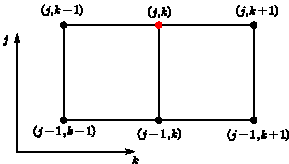
\includegraphics[width=0.5\textwidth]{assets/差分格式示意图.pdf}
    \caption{\textbf{向后加权隐式差分结点示意图}}\label{向后加权隐式差分结点示意图}
\end{figure}
\end{definition}



\begin{definition}[三层显式格式(R格式、DF格式)]
“三层”是指时间项占据三层,对 $t$ 采用两点中心差分,对 $x$ 采用三点中心差分,即得 Richardson 格式,虽然经典,却是完全不稳定格式,如下:
\begin{equation}
    \frac{u_j^{k+1}-u_j^{k-1}}{2h_t}-a\frac{u_{j+1}^k-2u_j^k+u_{j-1}^k}{h_x^2}=0
\end{equation}

在 Richardson 格式基础上进行修正,得到 DuFort-Frankel 格式,它是无条件稳定的:

\begin{gather}
    \frac{u_{j}^{k+1} - u_{j}^{k-1}}{2h_t}=a\frac{u_{j+1}^{k}-(u_{j}^{k+1}+u_{j}^{k-1})+u_{j-1}^{k}}{h_x^2} \\ 
    \Longleftrightarrow    u_{j}^{k+1} = \frac{1}{2} \left(u_{j+1}^k + u_{j-1}^k + \frac{h_t}{h_x^2}(u_{j+1}^{k-1} - u_{j-1}^{k-1}) \right)
\end{gather}

\end{definition}


\begin{definition}[三层隐式格式]

将CN格式的两个时间层推广到三个时间层,所得隐式格式为:
\begin{equation}
    \frac{u_j^{k+1}-u_j^{k-1}}{2h_t}=a\frac{1}{3h^2}(\delta_x^2u_j^{k+1}+\delta_x^2u_j^k+\delta_x^2u_j^{k-1})
\end{equation}

其截断误差为 $O(h_t^2 + h_x^2)$,且是无条件稳定格式。

\end{definition}


\begin{definition}[预测-校正格式]
\end{definition}


\begin{definition}[不对称格式]
\end{definition}


\section{对流扩散方程}


\begin{definition}[对流扩散方程]

当对流和扩散都存在时,如边界层流动,就要考虑对流扩散方程,如Brugres方程:

\begin{equation}
    \frac{\partial u}{\partial t}+u\frac{\partial u}{\partial x}=\nu\frac{\partial^{2}u}{\partial x^{2}}
\end{equation}

对流与扩散达到平衡时,有边界条件:

\begin{equation}
    u(0,t)=u_{0},\ u(L,t)=0\ \text{,也即} \ u(x_0,t)=u_{0},\ u(x_e,t)=0
\end{equation}

\end{definition}


\section{二维热传导方程}


\begin{definition}[二维热传导方程]

现讨论二维热传导方程的差分格式:

\begin{equation}
    \frac{\partial u}{\partial t}=\frac{\partial^2u}{\partial x^2}+\frac{\partial^2u}{\partial y^2},\quad(x,y)\in\Omega 
\end{equation}

\end{definition}


\begin{definition}[向前加权差分格式]

对 $t$ 采用向前差分格式,对 $x$ 和 $y$ 采用(向前)加权中心差分格式,这样可以得到多种显式或隐式格式:

\begin{equation}
    \begin{aligned}
        \frac{u_{i,j}^{k+1}-u_{i,j}^{k}}{h_t}& =\frac{\theta_{1}}{h^{2}}(u_{i+1,j}^{k+1}-2u_{i,j}^{k+1}+u_{i-1,j}^{k+1})+\frac{1-\theta_{1}}{h^{2}}(u_{i+1,j}^{k}-2u_{i,j}^{k}+u_{i-1,j}^{k})  \\
        &+\frac{\theta_{2}}{h^{2}}(u_{i,j+1}^{k+1}-2u_{i,j}^{k+1}+u_{i,j-1}^{k+1})+\frac{1-\theta_{2}}{h^{2}}(u_{i,j+1}^{k}-2u_{i,j}^{k}+u_{i,j-1}^{k})
    \end{aligned}
\end{equation}

也即:

\begin{equation}
    \frac{u_{i,j}^{k+1}-u_{i,j}^{k}}{h_t} = \theta_1\frac{\delta^2_x u_{i,j}^{k+1}}{h_x^2} + (1- \theta_1)\frac{\delta^2_x u_{i,j}^{k}}{h_x^2} + \theta_2\frac{\delta^2_y u_{i,j}^{k+1}}{h_y^2} + (1- \theta_2)\frac{\delta^2_y u_{i,j}^{k}}{h_y^2}
\end{equation}

\end{definition}

例如,令 $\theta_1 = \theta_2 = 0$,可得截断精度 $O(h_t + h_x^2 + h_y^2)$,稳定性条件为 $h_t\leqslant\frac{1}{2\left(\frac{1}{\Delta x^{2}}+\frac{1}{\Delta y^{2}}\right)}$ 的差分格式。


\begin{definition}[Saul'yev 不对称格式]
\end{definition}


\begin{definition}[DuFort-Frankel格式]

一维DuFort-Frankel 方法可推广到二维,首先写出二维 Richardson 格式(对时间采用两点中心差分,对空间采用三点中心差分),改格式为无条件不稳定格式,然后作替换 $u_{i,j}^{k} \longmapsto \frac12(u_{i,j}^{k+1}+u_{i,j}^{k-1})$,即得 DuFort-Frankel 格式:

\begin{gather}
    \frac{u_{i,j}^{k+1}-u_{i,j}^{k-1}}{2h_t}=\frac{u_{i+1,j}^k+u_{i-1,j}^k-u_{i,j}^{k+1}-u_{i,j}^{k-1}}{h_x^2}+\frac{u_{i,j+1}^k+u_{i,j-1}^k-u_{i,j}^{k+1}-u_{i,j}^{k-1}}{h_y^2} \\ 
    \Longleftrightarrow    u_{i,j}^{k+1}= \frac{1}{\frac{1}{2} + \frac{h_t}{h_x^2} + \frac{h_t}{h_y^2}} \left[\frac{h_t}{h_x^2}(u_{i+1,j}^{k}+u_{i-1,j}^{k})  + \frac{h_t}{h_y^2}(u_{i,j+1}^{k}+u_{i,j-1}^{k}) + (\frac{1}{2} - \frac{h_t}{h_x^2} - \frac{h_t}{h_y^2})u_{i,j}^{k-1} \right] \label{公式6}
\end{gather}

该式是显式格式,截断误差 $O(h_t^{2}+h_x^{2} + h_y^2 +\frac{h_t^{2}}{h_x^{2}} + \frac{h_t^{2}}{h_y^{2}})$,且无条件稳定。计算时,需要已知两个时间层上的值,其中 $k = 0$ 上的值由初始条件给出,$k = 1$上的值由前面其他公式或 $\frac{1}{2} - \frac{h_t}{h_x^2} - \frac{h_t}{h_y^2} = 0$(例如 $h_t = \frac{h_x^2}{4} = \frac{h_y^2}{4 }$ ) 时的公式 \ref{公式6}  来计算。



\end{definition}














































































































































































































































































































































































































































































































































































































\end{document}

% VScode 常用快捷键:

% F2:                       变量重命名
% Ctrl + Enter:             行中换行
% Alt + up/down:            上下移行
% 鼠标中键 + 移动:           快速多光标
% Shift + Alt + up/down:    上下复制
% Ctrl + left/right:        左右跳单词
% Ctrl + Backspace/Delete:  左右删单词    
% Shift + Delete:           删除此行
% Ctrl + J:                 打开 VScode 下栏(输出栏)
% Ctrl + B:                 打开 VScode 左栏(目录栏)
% Ctrl + `:                 打开 VScode 终端栏
% Ctrl + 0:                 定位文件
% Ctrl + Tab:               切换已打开的文件(切标签)
% Ctrl + Shift + P:         打开全局命令(设置)

% Latex 常用快捷键

% Ctrl + Alt + J:           由代码定位到PDF
% 


% Git提交规范:
% update: Linear Algebra 2 notes
% add: Linear Algebra 2 notes
% import: Linear Algebra 2 notes
% delete: Linear Algebra 2 notes